\chapter{Tervezés}

\section{Az alkalmazás fejlesztés bemutatása}

Az Androidos alkalmazás, vagyis az e-Horgásznapló egy Android operációs rendszeren futó, adat rögzítésre használatos alkalmazás. Célom az egyszerű, felhasználóbarát kezelőfelület, ahol a lehető legegyszerűbben rögzíteni tudja a horgász a kifogott hal adatait, és a fogás helyszínét.
Az alkalmazást Android Studio segítségével fogom elkészíteni Kotlin segítségével a könnyebb átláthatóság, és kevesebb boilerplate\cite{boilerplate} kód miatt. Az alkalmazásom a korábban használt Model-View-controller fejlesztési elv helyett az új Model-View-ViewModel architektúrát használja, ezáltal az alkalmazás jövő állóbb.


\section{Model-View-ViewModel}

Ahogy az előző szekcióban említettem az alkalmazásom a Model-View-ViewModel architektúrát alkalmazza. Ennek a mintának az a célja, hogy elkülönítse az alkalmazás logikai rétegeit, így egyszerűbb lesz a kód karbantarthatósága, és újra használása. Ebben különösen segítségünkre lesz a nemrég bevezetett Jetpack Compose, ami a régi XML elrendezést hivatott leváltani.

A MVVM-nek\cite{mvvm} három fő része van:
\begin{itemize}
    \item Model: Az adatokat, és a logikát tartalmazó réteg.
    \item View: A felhasználói felület.
    \item ViewModel: Köztes réteg, ez köti össze a Model-t, és a View-t. Feladata az adatok feldolgozása, és kezelése.
\end{itemize}

\begin{figure}[h]
\centering
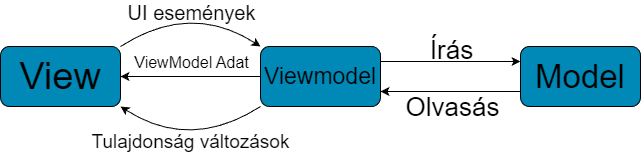
\includegraphics[scale=0.6]{images/mvvm2.png}
\caption{MVVM architektúra diagram}
\label{fig:mvvm}
\end{figure}

\subsection{Model}

A Model az alkalmazás adatait és üzleti logikáját tartalmazza. Ide tartoznak az olyan elemek, mint az adatbázisok, a hálózati API-k, vagy a fájlkezelés. A Model réteg az adatforrások elérését és az adatok frissítését biztosítja, de nem tartalmaz semmilyen logikát a felhasználói felülethez.

\subsection{View}

A View az a réteg, amely a felhasználói felületet kezeli. Ez felelős az adatok megjelenítéséért és a felhasználói bevitelek kezeléséért. A View réteg nem tartalmaz logikát az adatok feldolgozására; csak megjeleníti az adatokat, amelyeket a ViewModel szolgáltat számára.

\subsection{ViewModel}

A ViewModel az MVVM minta központi eleme, amely kommunikál a Model és a View között. A ViewModel adatokat kér a Modelltől, feldolgozza azokat, és úgy adja át a View-nak, hogy azok egyből megjeleníthetők legyenek. A ViewModel általában LiveData objektumokat használ, amelyek lehetővé teszik, hogy az adatok automatikusan frissüljenek a View-ban, ha változás történik bennük.

\section{A program felépítése}

A MVVM architektúra kulcsfontosságú szerepet fog betölteni az alkalmazásunkban. Mivel ezen szemlélet alapján kezdem el az alkalmazást, fontos hogy a \textbf{mindsk 21} (minimum Operációs rendszer követelmény) legyen beállítva. Ez jelen esetben az Android 5-ös verziót jelenti. 

A programban egyszerűségre törekszek, hogy minél szélesebb felhasználó közönség igénybe tudja venni a programot. Fontos, hogy intuitív, és letisztult legyen a kezelői felület, a lehető legkevesebb hibalehetőség merüljön fel a User részéről. Ezért a programom felépítését az alábbiak szerint képzelem el:

\begin{figure}[h]
\centering
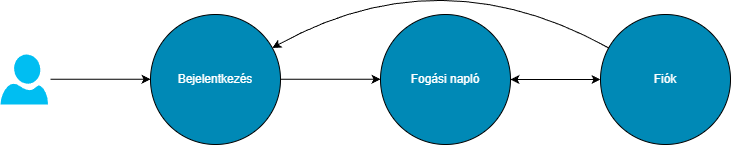
\includegraphics[scale=0.6]{images/userdiagram.png}
\caption{felhasználói diagram}
\label{fig:userdiagram}
\end{figure}

A felhasználó az applikáció megnyitása után a bejelentkezés kijelzőre lesz irányítva, ahol be tud jelentkezni ideális esetben a MOHOSZ-nál regisztrált adataival. Miután ez megtörtént át lesz irányítva a fogási napló oldalra, ahol látni fogja az összes fogását időrendi sorrendben. 

\vspace{1cm}

Ezen a ponton tudja feltölteni a legfrissebb fogását a naplóba, ahol a következőket kell megadnia:
\begin{itemize}
    \item Tó neve
    \item Tó víztérkódja
    \item Hal neve
    \item Hal súlya
\end{itemize}

Ezután az alkalmazás automatikusan hozzárendeli a \textbf{SystemDate} változót, így elkerülve a különböző csalásokat, későbbi fogás hozzáadásokat a rendszerben. Tehát a felhasználó nem adhatja meg a fogásának az időpontját.

A fogás rögzítése után a rendszer hozzárendeli az adatbázishoz az éppen létrejött adatokat, és sorrend szerint legfelülre rakja. Itt megtekinthetjük a frissen hozzá adott fogást a régebben hozzáadotakkal együtt.

Ezen a ponton felmerülhet egy kérdés, hogy mi a helyzet akkor, hogyha úgy döntött egyik horgásztársunk, hogy a vízpartra mindenféle okos eszköz érkezik meg?
Itt jön szóba a fiók oldal, ahol ezt a problémát lenne érdemes orvosolni.

A fogási napló tetején egy \textbf{TopBar} változóval hozzárendelünk egy gombot, ami átvezet minket a fiók fülre, ahol megtekinthetjük az éppen bejelentkezett egyént, és felkínáljuk a lehetőséget a kijelentkezésre. Ezután az alkalmazás vissza vezet minket a bejelentkezés fülre, ahol sport társunk bejelentkezhet saját fiókjával, és nyomon követheti, illetve naplózhatja fogásait.

\subsection{Bejelentkezés}

Előszöri belépésnél a felhasználónak megoldást kell kínálni a bejelentkezéshez, amit nem lehet fél vállról venni. Minden alkalmazásban megadott adat szenzitív, alapos körültekintéssel kell ezeket kezelni. Mivel fejlesztő környezetnek az Android Studio-t választottam a különböző Google által fejlesztett API-k könnyen integrálhatóak az alkalmazásba. Ezt kihasználva hosszas tanakodás után a Firebase tűnik a legmegfelelőbb választásnak. 

A Firebase felhőszolgáltatást nyújt nekünk kölünböző előre létrehozott API-kal, amik gördülékenyebbé teszik az alkalmazás fejlesztés ezen szakaszát. Természetesen a bejelentkezésre is nyújt egy külön megoldást, aminek a neve \textbf{Firebase Authentication}\cite{firebaseauthentication}. Ezzel az API-val dolgozva csak meg kell adnunk a bejelentkezés típusát, és máris neki állhatunk az alkalmazásba való beépítésnek. Itt fontos megemlíteni, hogy ez a szolgáltatás nem teljesen ingyenes, csak egy bizonyos erőforrás kapacitás használatáig, azonban a mi esetünkben az alkalmazás méretét tekintve nem befolyásoló tényező.

A bejelentkezés a Firebase integrációja után így nézne ki:
\begin{itemize}
    \item E-mail beviteli mező
    \item Jelszó beviteli mező
    \item Bejelentkezés gomb
\end{itemize}

A bejelentkezés gomb megnyomása után ellenőrizni tudjuk, hogy a felhasználó által, vagy általunk által megadott bejelentkezési információk megegyeznek-e az adatbazisban szereplő értékekkel. 

\begin{figure}[h]
\centering
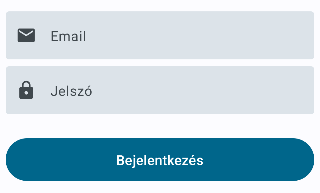
\includegraphics[scale=1]{images/login.png}
\caption{A bejelentkezés panel egy elképzelt változata.}
\label{fig:loginpanel}
\end{figure}

\subsection{A fogási napló}

Mituán bejelentkezett a User szeretném, ha egyből a fogási napló oldalon találná magát. 
Az alkalmazás elemi része továbbra is az egyszerűség, így a könnyű felhasználást szeretném ezzel elősegíteni. Mivel itt adatokat fogunk tárolni szükségünk van valamilyen adatbázisra.
Erre a célra az Android studio-ban integrált \textbf{Room}\cite{room} adatbázist fogom használni, ami egyszerűen lokálisan tárolja a felhasználó által feltölteni kívánt adatokat.
Ezen a ponton szeretném, ha sima felsorolás nézetben megtudja tekinteni a felhasználó az eddigi fogásait az alábba szempontok szerint:
\begin{itemize}
    \item Fogás időpontja
    \item Fogás helye
    \item A tó víztérkódja
    \item Hal típusa
    \item Hal súlya
\end{itemize}

A képernyő jobb alsó sarkában ésszerű lenne egy \textbf{FloatingActionButton}, ami az adatfelvitel \textbf{Dialog}-ra vezetne át minket, ahol feltölthetjük az adatainkat.

A fogás időpontja a korábban említett \textbf{Systemdate} változó lenne, amit nem tudunk megváltoztatni, mindig a fogás rögzítésének ideje szerepel.
A fogás helye természetesen a tó neve lenne, ami egy \textbf{String} változó, itt begépelhetjük az éppen kikapcsolódás céljával használatba vett vizet.
A tó víztérkódja nem elfelejthető adat, ez \textbf{Int} változó lenne.
A hal típusa, pontosítva a hal neve egy \textbf{String} változó lenne, ahogy megadhatjuk a fogott halunk nevét.
Végül a hal súlya értelemszerűen a mérlegelés után megállapított szám avagy \textbf{Int}, kilogramm-ban.

\subsection{Fiók}

Az utolsó szekció a fiók oldal, ami azt szolgálná, hogy a felhasználó ki tudjon jelentkezni az alkalmazásból, lehetőséget biztosítva egy másik fiók bejelentkezésére, vagy ugyanazzal az adatokkal való vissza-jelentkezésre.

Itt biztosítani kell a felhasználónak egy kijelentkezés gombot, amivel kijelentkezik a fiókjából, és visszatér a bejelentkezés oldalra. 

Továbbá egy másik lehetőséget is érdemes felkinálni a felhasználónak, ahol visszatud térni a fogási napló oldalra.